\section{Introduction}
\label{sec:intro}

When we cannot check an answer, we often ask a second opinion.
The same intuition now runs through many LLM pipelines.
Panels of models act as evaluators~\citep{verga2024juries}, ensembles vote on labels and answers~\citep{li2024moreagents,jiang2023llmblender}, and agreement across samples is used to detect hallucinations and to pick answers~\citep{wang2023selfconsistency}.
All of these practices assume that {\em consensus implies correctness}.

This assumption matters most where labels are scarce and decisions are value-laden.
If model errors were independent, agreement among several models would be strong evidence of a correct answer.
But models are trained on overlapping data with similar objectives, and recent work shows that their errors are strongly correlated~\citep{goel2025greatmodels,kim2025correlated}.
Shared errors are especially worrying for ethical judgement.
There, models may share leanings learned from pre-training data and alignment, and the reference labels themselves reflect one group's norms~\citep{hendrycks2021ethics}.
In that setting, a confident consensus could be confidently wrong.

Prior work has studied pieces of this question in isolation.
On one hand, self-consistency shows that agreement {\em within} one model predicts correctness on math~\citep{wang2023selfconsistency}, and multi-agent voting reports accuracy gains~\citep{li2024moreagents}.
On the other hand, studies of correlated errors measure similarity between models but do not ask how well agreement works as a correctness signal in each domain.
What is missing is one controlled comparison on {\em the same model pool} that measures (a) how strongly agreement tracks correctness, (b) whether a majority vote beats the best single model, and (c) how well agreement separates right from wrong answers without labels, across factual, math and ethics tasks.

Our main question is: {\bf how much does inter-model agreement tell us about correctness, and is it a weaker signal for ethics?}
We hypothesize that agreement correlates with correctness at $r \in [0.4, 0.6]$ on factual and math tasks but at $r < 0.2$ on ethics, that a vote of five or more models beats the best model by 3--7\pp on factual QA but not on ethics, and that agreement alone reaches AUROC 0.70--0.80 on factual tasks.
To test this, we run 8 open-weight instruction models from 7 developer families on 7 tasks of 500 items each.
The tasks cover open-ended trivia (\triviaqa), multiple-choice knowledge (\mmlu), math word problems (\gsm), competition math (\mathfive) and two \ethics subsets.
We also add a control: \mmlutf, a {\em binary} true/false version of \mmlu.
It matches the two-way answer format of \ethics, which lets us separate the effect of the ethics domain from the effect of a binary answer space.

We find that agreement is a strong label-free signal on factual and math tasks (AUROC 0.78--0.91), and that the plurality answer is correct 96--100\% of the time when all 8 models agree on open-ended tasks (\figref{fig:calibration}).
On ethics the signal is clearly weaker (AUROC 0.63--0.71).
However, about half of this gap comes from answer format: the binary factual control (AUROC 0.735) is statistically indistinguishable from \ethics commonsense (0.711, $p=0.48$).
The domain-specific part of the story lies in the vote.
On ethics, model errors are more correlated than on the control (mean pairwise $\phi$ 0.45--0.49 vs.\ 0.30).
The plurality vote is significantly worse than the best model ($-4.8$\pp, Holm $p=0.008$), and this deficit grows from $-1.3$\pp to $-4.8$\pp as the ensemble grows from 3 to 8 models.
Contrary to our hypothesis, voting also fails to beat the best model on factual QA ($-1.8$ to $-2.4$\pp, not significant) and helps only on math ($+2.0$ to $+2.4$\pp).

\begin{figure}[t]
    \centering
    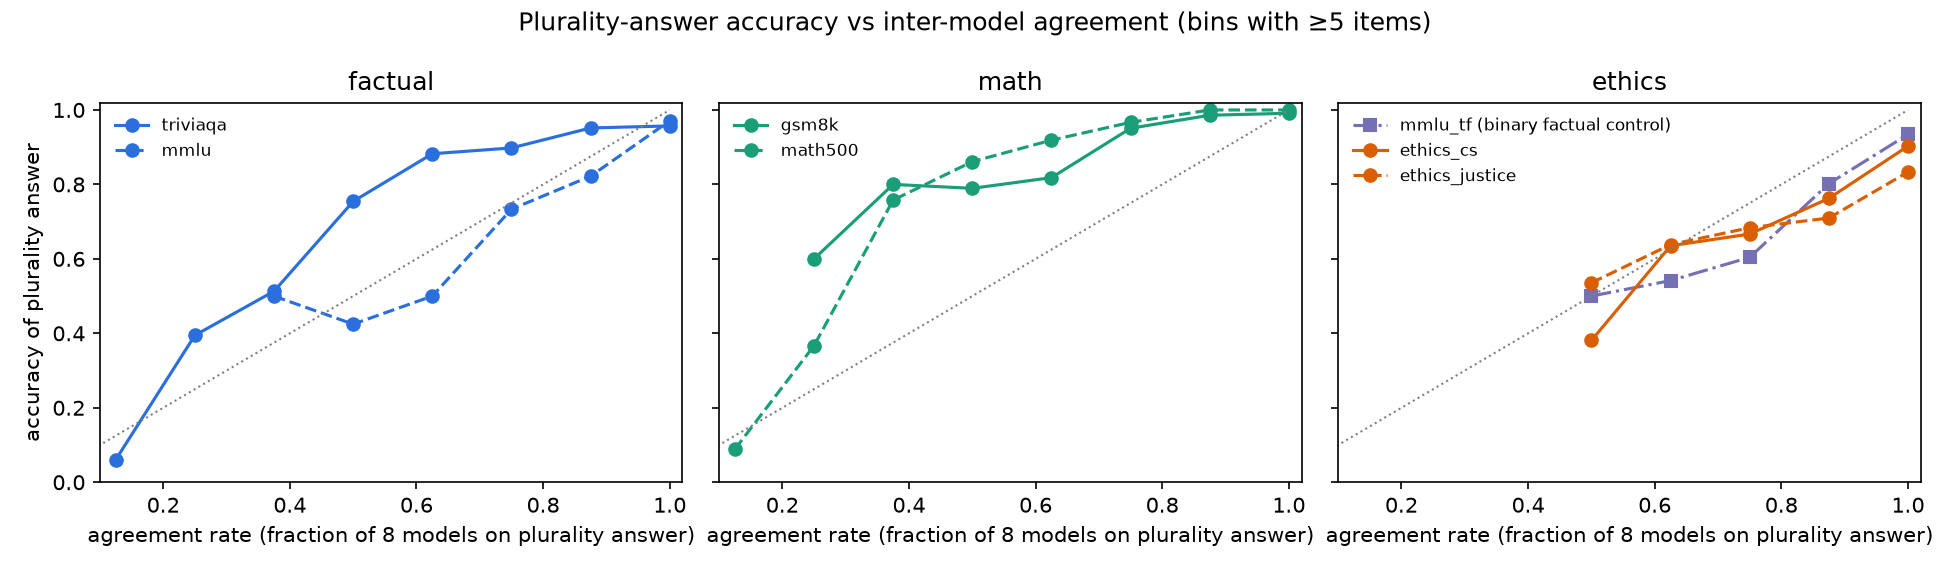
\includegraphics[width=0.98\linewidth]{figures/agreement_vs_accuracy.png}
    \caption{Accuracy of the plurality answer as a function of inter-model agreement (fraction of 8 models giving the plurality answer; bins with $\geq$5 items; dotted line is the diagonal).
    On factual and math tasks, accuracy rises steeply with agreement and approaches 1 at full agreement.
    On ethics, items concentrate at high agreement, yet accuracy stays at 0.83--0.90 even when all 8 models agree.
    The binary factual control (\mmlutf, purple) follows a similar curve to the ethics tasks, which shows that part of the weakness comes from the binary answer format.}
    \label{fig:calibration}
\end{figure}

In summary, our contributions are:
\begin{itemize}[leftmargin=*,itemsep=0pt,topsep=0pt]
    \item We conduct a controlled, cross-domain study of inter-model agreement as a correctness signal on 3,500 items, with 8 models from 7 families answering every item.
    \item We introduce a format-matched binary factual control and show that roughly half of the factual-vs-ethics gap in AUROC is due to answer format rather than domain.
    \item We show that agreement-based ranking and majority voting behave differently. Agreement ranks items well everywhere, but the vote beats the best model only on math, and on ethics its deficit grows with ensemble size, as correlated errors would predict.
    \item We analyze unanimous-but-wrong cases and find that ethics consensus errors combine crowd-label noise with systematic shared model leanings, while factual consensus errors are rare: only 0.4--2.2\% of open-answer and math items have $\geq$75\% agreement on a wrong answer.
\end{itemize}

\Secref{sec:related} reviews related work, \secref{sec:method} describes the setup, \secref{sec:results} presents results, \secref{sec:discussion} discusses implications and limitations, and \secref{sec:conclusion} concludes.
